% ---------------------------------------------------
% ----- Chapters of the template
% ----- for Bachelor-, Master thesis and class papers
% ---------------------------------------------------
%  Created by C. Müller-Birn on 2012-08-17, CC-BY-SA 3.0.
%  Freie Universität Berlin, Institute of Computer Science, Human Centered Computing. 
%
% TODO remove 2 - to use auto numbering
\chapter{4 - User research and analysis}
\label{chap:chapters} 


To prevent the common problem in software development, where instead of relying on meaningful user input quickly building on ideas of individual stakeholders who might never even use the product,
I wanted to apply diffrent methods of user research commonly used in HCI, and evaluate how helpful they prooved in the context laid out earlier.
\\
The process used for this project abstractly looks as following:


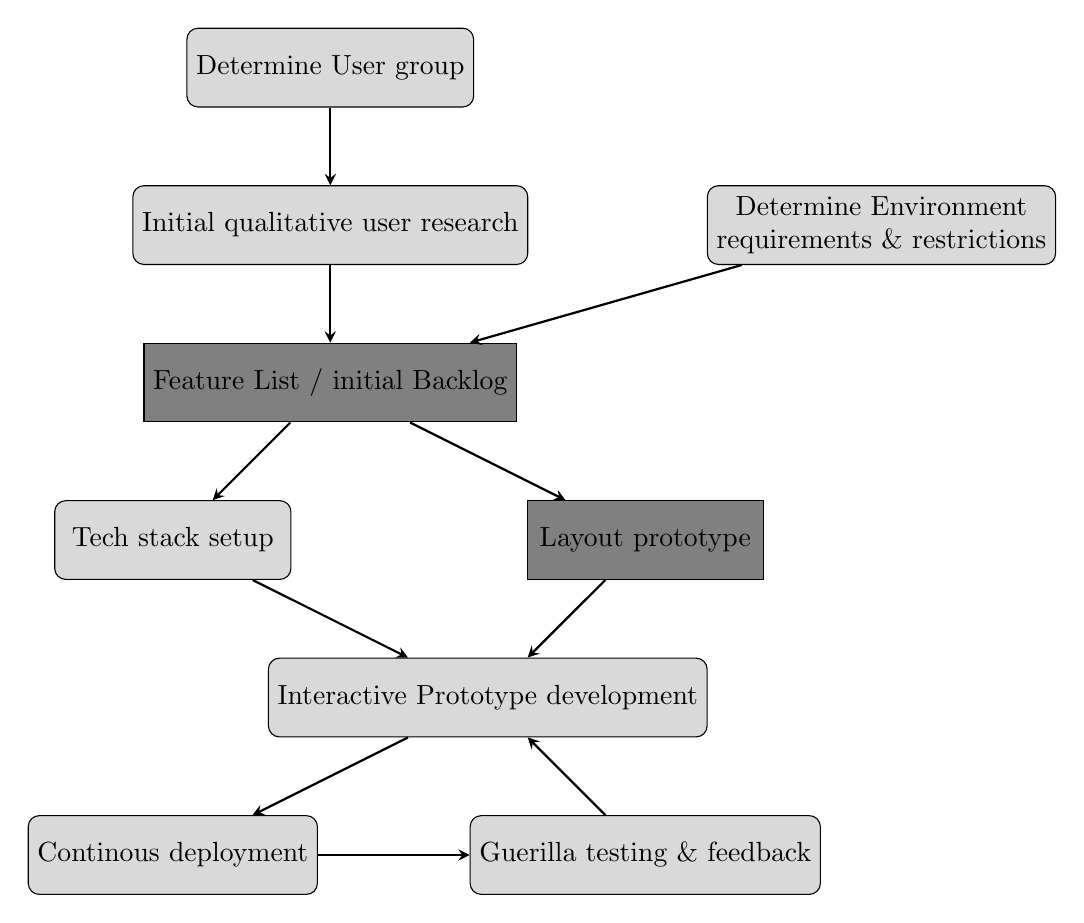
\begin{tikzpicture}[node distance=2cm]
  \tikzstyle{round} = [rectangle, rounded corners, minimum width=3cm, minimum height=1cm,text centered, draw=black, fill=gray!30]
  \tikzstyle{rect} = [rectangle, minimum width=3cm, minimum height=1cm,text centered, draw=black, fill=gray]
  \tikzstyle{arrow} = [thick,->,>=stealth]

  \node (dug) [round] {Determine User group};
  \node (interview1) [round, below of=dug] {Initial qualitative user research};
  \node (denv) [round, right of=interview1, xshift=5cm, align=center] {Determine Environment\\requirements \& restrictions};
  \draw [arrow] (dug) -- (interview1);
  \node (bl) [rect, below of=interview1] {Feature List / initial Backlog};
  \draw [arrow] (denv) -- (bl);
  \draw [arrow] (interview1) -- (bl);
  \node (tech1) [round, below of=bl, xshift=-2cm] {Tech stack setup};
  \node (layout) [rect, right of=tech1, xshift=4cm] {Layout prototype};
  \draw [arrow] (bl) -- (tech1);
  \draw [arrow] (bl) -- (layout);
  \node (proto) [round, below of=tech1, xshift=4cm] {Interactive Prototype development};
  \draw [arrow] (tech1) -- (proto);
  \draw [arrow] (layout) -- (proto);
  \node (deploy) [round, below of=proto, xshift=-4cm] {Continous deployment};
  \draw [arrow] (proto) -- (deploy);
  \node (feedback) [round, right of=deploy, xshift=4cm] {Guerilla testing \& feedback};
  \draw [arrow] (deploy) -- (feedback);
  \draw [arrow] (feedback) -- (proto);
\end{tikzpicture}
  